\documentclass[11pt]{article} %This sets the font size and the document class of your report. In this case we use 'article' as that is ideal for shorter reports.
\usepackage{amssymb}
\usepackage{amsmath}
\usepackage{subcaption}
% LaTeX can be enhanced by the use of packages. These packages can do many things, a few of the most common and useful are used here. They are declared before the document proper, in what is known as the 'preamble'. Packages need to be installed when a .tex file compiles into a .pdf, but should do so automatically.
\usepackage[top=1.5cm, bottom=1.5cm, left=1.75cm, right=1.75cm]{geometry} %This sets the margins of the report.

\usepackage{graphicx} % A package allowing insertion of images into the text.
\usepackage{caption}
\usepackage{rotating}

% Choose your citations style by commenting out one of the following groups. If you decide to change style, you should also delete the .bbl file that you will find in the same folder as your .tex and .pdf files.

% IEEE style citation:
\usepackage[style=ieee]{biblatex}
\addbibresource{Solution.bib}

\usepackage{enumerate}
\usepackage{enumitem}
%% Author-date style citation:
%\usepackage[round]{natbib} % A package that creates references in the author-date style, with round brackets
%\renewcommand{\cite}{\citep} % For use with natbib only: comment out for the cite package.
%\bibliographystyle{plainnat} % Author-date referencing (use in conjunction with the natbib package)
\usepackage{color} % Allows the colour of the font to be changed by using the '\color' command: This is just to support the blue comments in this template...use standard (black) text in your report.
\usepackage{float}
\usepackage{subdepth}
\usepackage{mathtools}
\usepackage{tabularx}
\usepackage{makecell}
\linespread{1} % Sets the spacing between lines of text.
\setlength{\parindent}{0cm}  % Suppresses indentation of text at the start of a paragraph
\pagenumbering{arabic} % sets the style of page numbering for the report


\begin{document} % This begins the document proper and ends the pre-amble

% The last } finishes the chunk of text opening with {\color{blue}..., so all of the above appears as blue text. A common LaTeX error is to forget to close such a chunk of text, so if the formatting goes wrong look for a missing }.

% To get rid of the blue text, select and delete everything from '{\color' to '}', inclusive, leaving \ begin{titlepage} as the first command  after \begin{document}

\begin{center} % Starts the beginning of an environment where all text is centered.

{\Huge Battleship Board Game}\\[0.5cm] % [0.5cm] sets the distance between this line and the next.
\vspace{5mm}
\textit{Enrico Zammit Lonardelli}
\\
\vspace{5mm}
\text{9910821}
\\
\vspace{5mm}
\text{School of Physics and Astronomy}
\\
\vspace{5mm}
\text{The University of Manchester}
\\
\vspace{5mm}
\text{PHYS30782: Object-Oriented Programming in C++}
\\
\vspace{5mm}
\text{May 2020}
\\
\end{center}
\vspace{10mm}
\section{Introduction}
\subsection{Choice of game motivation}
The board game Battleship I chose to reproduce digitally is inspired from the early 20th century pencil and paper game which later
became a success board game hit in the early 1960s.
This board game in particular has always had a connection with the computer world, in fact being one of the world's ever
computer games being released in 1979 on the Z80 Compucolor \cite{hinebaugh2009board}.
Since then this game has been reproduced on many digital consoles and as a standalone game on PC and is a game I have personally played many
times as a child so I decided it would be a good idea to reproduce a command-line version of it in C++.
\subsection{Rules}
The rules followed are according to the original Hasbro board game rules \cite{rules} with the exception of a
raft instead of a destroyer ship.
The game is played by two players.
Each player has access to two grids representing their positioning of ships and the opponents' guess positions.
At the start of the game each player has access to the following types ships:
\begin{table}[!h]
\centering
\begin{tabular}{c|c|c}
Name & Horizontal Length & Appearance \\
\hline
Carrier & 5 & \verb|<-+->| \\
Cruiser & 4 & \verb|<++>| \\
Destroyer & 3 & \verb|<+>| \\
Submarine & 3 & \verb|<*>| \\
Raft & 2 & \verb|<>| \\
\hline
\end{tabular}
\caption{Table listing the pieces each player must have on the board.}
\label{table:pieces}
\end{table}
Once the battle begins, the first player enters a coordinate they would try to send a missile to on the
enemy's board.
If the coordinate is populated by a ship, that player must say "Hit!" otherwise they must say "Miss".
Depending on the outcome, the attacking player will update their enemy's guess board with the event.
The other player then has the attacking turn and this is repeated until one of the players is hit on their last
coordinate of their last ship.
\subsection{Program Requirements}
The following are the objectives set out at the beginning of the project to be completed by the end of project:
\begin{enumerate}[label=\Roman*.]
  \item The program \textbf{shall}:
  \begin{enumerate}[label=\arabic*.]
    \item allow a human player to have their own, unique account
    \item allow a human player to log in/out
    \item allow a human player to start a battle from the menu
    \item allow a human player to play against a computer-controlled player
    \item have a computer-controlled player able to randomly select a move on their turn
    \item enforce board game rules during the battle
    \item recognize when the game ends and save highscores if applicable
    \item have a navigable menu
    \item allow a human player to view fleet through the menu
    \item allow a human player to edit fleet through the menu
    \item allow a human player to save fleet settings across games
    \item allow a human player to view top 10 all-time game highscores through the menu
    \item allow a human player to exit the game
  \end{enumerate}
  \item The program \textbf{shall not}:
  \begin{enumerate}[label=\arabic*.,resume]
    \item throw uncaught errors exiting unexpectedly
    \item have memory leaks
  \end{enumerate}
  \item The program \textbf{may}:
  \begin{enumerate}[label=\arabic*.,resume]
    \item allow a human player to secure their account using a hashed password
    \item implement a smarter than random computer-controlled player
  \end{enumerate}
\end{enumerate}
\section{Code Design and Implementation}
This program was run and tested using gcc version 6.3.0 on a x86\_64-linux-gnu target running 'Debian 6.3.0-18+deb9u1' with GNU Make 4.1.
The make file in the src/ directory includes all the options needed and running 'make' in this directory followed
by moving to the build/ directory and running ./battleship will execute the program.
For a fully detailed documentation (not required but makes it easier for the reader)
 and how to access it please refer to instructions in Appendix 2.
Please note that most of the commenting explaining method motivation resides in
the respective header files.
\subsection{Navigation and Input Validation}
\begin{figure}[H]
\centering
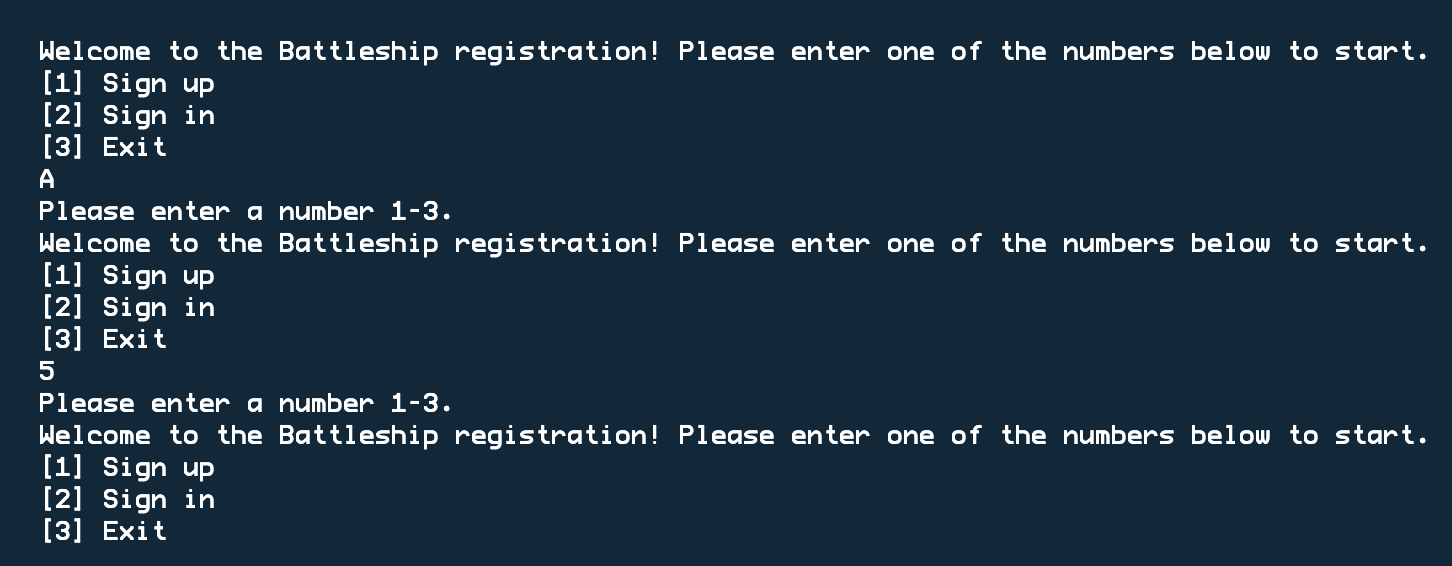
\includegraphics[scale=0.6]{images/input_validation.png}
\caption{Screenshot of the terminal illustrating input validation on menu input.}
\label{fig:input_validation}
\end{figure}
The navigation for this program is achieved through the use of menus (numbered lists) in the
command line interface.
The user is required to enter a number when prompted and press the 'Enter' key.
All menu input validation is done in two parts, first the std::cin failbit is checked after input
to check that the input was indeed a number.
Then the input is passed through a switch statement and the appropriate actions are taken.
Figure \ref{fig:input_validation} shows the error handling features.
\\
\par When the user is asked to input a coordinate later on in the game, this is done by
adding the std::istream as friend class to the battle\_ship::coordinates class.
A RegEx match on this input string is done to look for letters [A-J] and 1 to 2 digits.
The letter part is statically type casted to the battle\_ship::x\_axis enum class while the digit
is cast to a std::size\_t type.
A check is placed in case no letters and/or digits are found.
This ensures only valid letters and numbers are chosen.
One further check is applied to digits to check they are within range of the board [0,10).
If any of these checks do not pass, the user is notified and the method returns a falsy boolean
value which the calling method of this operator should read and act accordingly.
Figure \ref{fig:coordinate_validation} shows the error handling features of coordinate validation.
\begin{figure}[H]
\centering
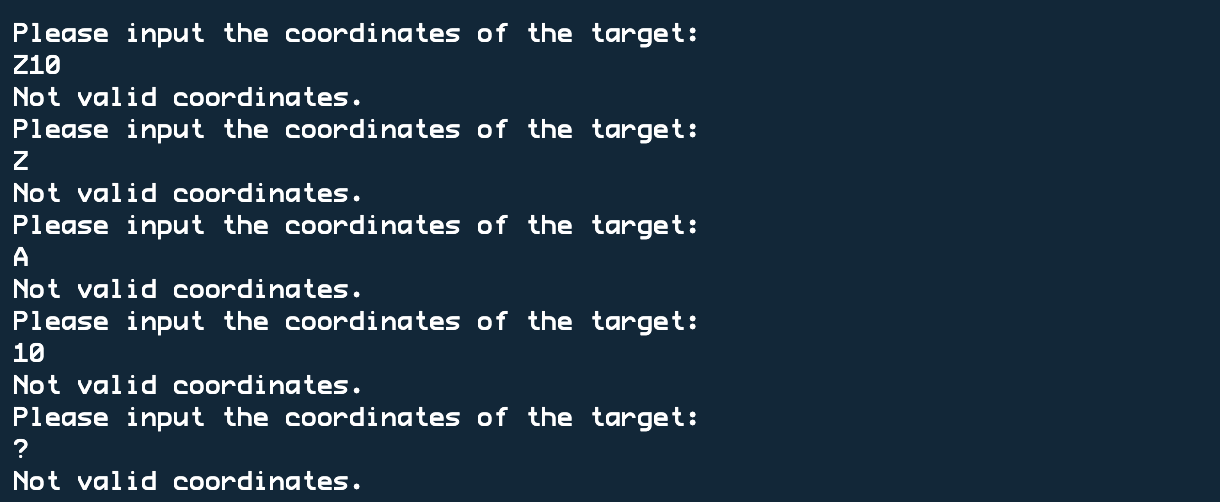
\includegraphics[scale=0.6]{images/coordinate_validation.png}
\caption{Screenshot of the terminal illustrating input validation on coordinates input.}
\label{fig:coordinate_validation}
\end{figure}
If in the edit fleet screen the user attempts to add a piece to the board which intersects with an already existing piece
the user should be notified and asked to choose another position.
The same logic although can be used when a player sets a target on their turn to send a missile
onto the enemy board.
For this reason, the battle\_ship::geometry class (seen later) was setup to check that no two pieces intersect.
\begin{figure}[H]
\centering
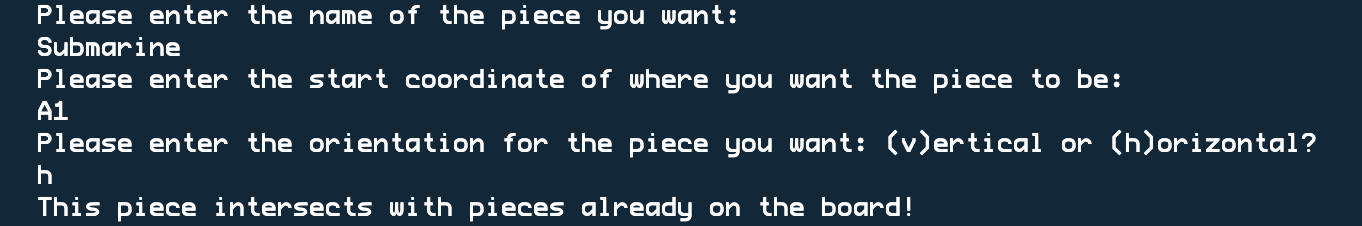
\includegraphics[scale=0.6]{images/board_validation.png}
\caption{Screenshot of the terminal illustrating input validation on a new piece input onto the board.}
\label{fig:board_validation}
\end{figure}
Lastly, Figure \ref{fig:all_menus} is a top-level flowchart of how the different menus are connected and
how what the user story is.
\begin{sidewaysfigure}[h]
\centering
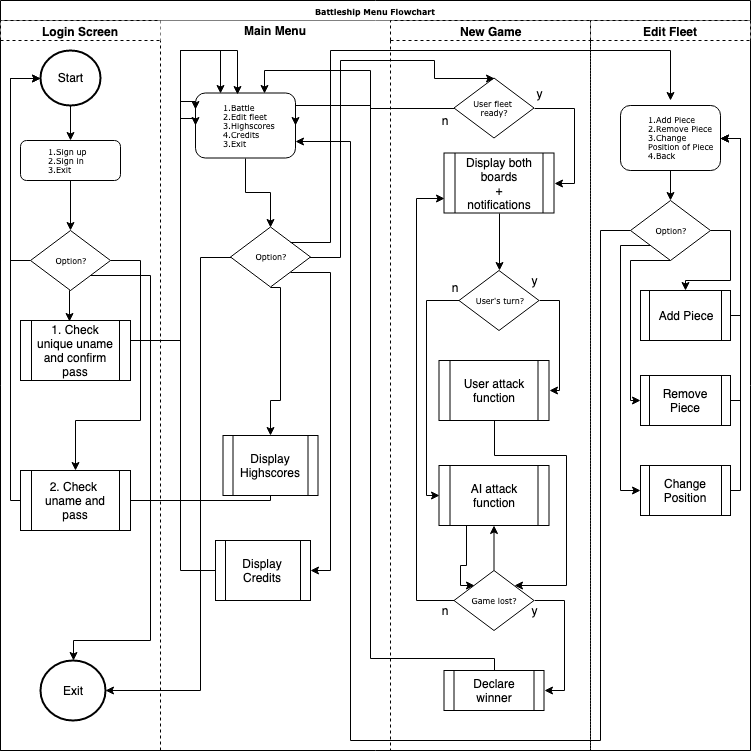
\includegraphics[scale=0.75]{images/menu.png}
\caption{Flowchart detailing how different menus and 'pages' are connected.}
\label{fig:all_menus}
\end{sidewaysfigure}
\clearpage
\subsection{Authentication}
The battle\_ship::authentication class was setup to handle signing in and up in the game.
The first special feature I used here is the use of the experimental/filesystem header file.
The filesystem header file is supposed to be included with C++17 however since I use gcc version 6
this still does not implement filesystem but it does have the Filesystem Technical Specification which is in
 experimental/filesystem. I use is std::experimental::filesystem::exists to check that the username
the user wishes to register with does not exist as a savefile already.
This single method call saves a lot code from having to loop through all the files
and checking them one by one.
\\
\par The other special feature in this class is from the std::functional header; the hash method.
This method accepts a key and applies a one way map which returns an std::size\_t number
representation for the key.
Only the same key will produce the same hash map output.
This is good security practice (not the best) to avoid saving passwords in plain text.
Instead we save the password hash to a user profile file and whenever the user needs to login we hash their input and compare hashes.
This way, the program never has to store passwords in clear text and does not explicitly have access to them.
\subsection{Class Hierarchies}
\subsubsection{Pieces}
\begin{figure}[H]
\centering
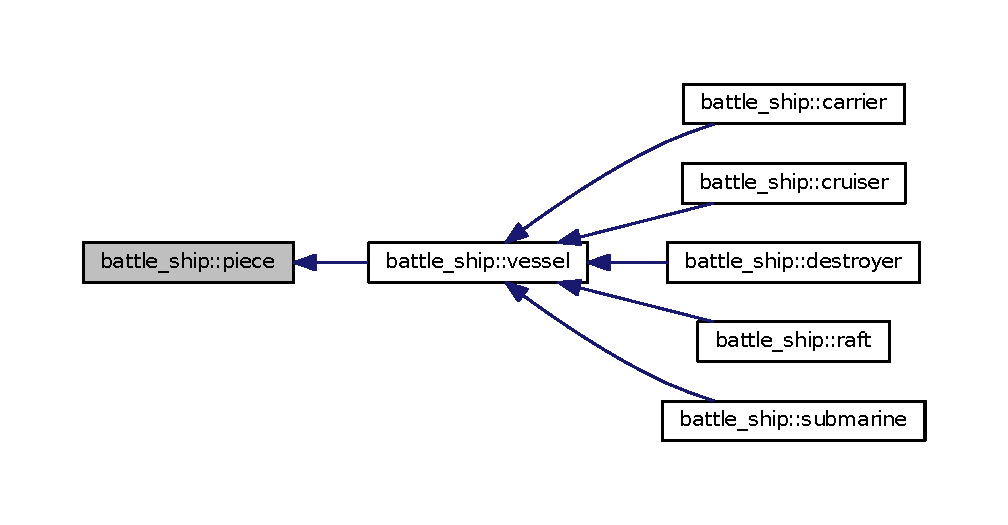
\includegraphics[scale=0.6]{images/piece.pdf}
\caption{Top level class diagram showing interface and inheritance hierarchy for the piece interface.}
\label{fig:piece_class_diagram}
\end{figure}
To make it easy to add new pieces to the game in the future and to maximise code reusability, the abstract class
battle\_ship::piece was created.
Moreover as per C.129 of the C++ Core Guidelines the design of the inheritance hierarchy needs careful attention.
I have implemented interface inheritance followed by implementation inheritance.
The former is providing an interface which is detached from implementation
to make it seemless when changing the actual logic of the methods for a particular implementor, without
affecting the other implementors or derived classes.
The latter is providing a base class which will allow derived classes to inherit its methods.
\\
\par My solution is to create the battle\_ship::piece class as an abstract class/interface defining all the methods its derived classes should implement.
This class has a number of pure virtual methods such as attribute getters and some methods to handle modifying the pose of the piece (position and orientation).
One important note is that this class does not declare any methods such as 'attack' since the thought is
in the future the needs might change and there might be non-attacking pieces such as decoys added to the game.
The class battle\_ship::vessel was declared to implement these methods.
This is a clear case of object oriented features such as inheritance explicitly as above
and polymorphism with the use of dynamic linkage of the pure virtual methods defined in the base interface and implemented in the derived battle\_ship::vessel class.
Individual ships defined in Table \ref{table:pieces} are then derived classes of battle\_ship::vessel.
They are further defined only through header files since the implementation is inherited and need only to pass different parameters to the base class constructor.
Finally, adding a new ship in the future is as easy as defining a new header class which calls the base class' constructor with the new properties defining this ship.

\subsubsection{Player}
\begin{figure}[H]
\centering
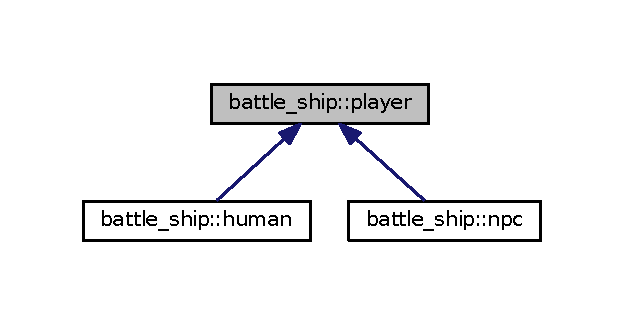
\includegraphics[scale=0.6]{images/player.pdf}
\caption{Top level class diagram showing inheritance hierarchy for the player base class.}
\label{fig:piece_class_diagram}
\end{figure}
There is another class hierarchy for the concept of a player in the game.
Requirement 4 in Section 1.3 requires the ability of the game to have a human player interact with a computer controlled one.
For this reason I chose to create the base class battle\_ship::player which does have pure virtual functions
however is not solely an interface and does have private data.
Through dynamic linkage and polymorphism methods such as the attack method are implemented by the derived classes
battle\_ship::human and battle\_ship::npc (Non-player character).
Through this hierarchy for example, the NPCs do not save their highscore while the humans do.
They also have different attack functions where in the human's case they are asked for the target
while in the NPC's case a random point is randomly selected when it is their turn (retrying only if the point had already been tried).

\subsection{Manager Classes}
I have implemented four classes known in the codebase as 'Manager Classes'.
The purpose of these classes is to manage certain aspects such as notifications, highscores, market and screen output.
Practically, these managers are used to hold data and methods frequently used by different classes through
leveraging static type member data and methods.
\\
\par The battle\_ship::screen\_manager class is used to produce the three columned output seen in the terminal
so that any notifications can be shown to terminal together with the current board view.
In this case it makes sense to use the static type member function since it would be unoptimized to
have to instantiate this class every time since no state needs to be maintained between calls anyways.
It contains a general, repeatedly used member function which needs to be accessible in different parts of the codebase.
With the same reasoning the battle\_ship::highscore\_manager does the same with no member data but just useful methods
which are used in other places of the code. This class uses an advanced C++ feature which is a generic lambda function
to custom sort a vector of tuples on the second element of that tuple.
\\
\par The battle\_ship::market\_manager is used for functionalities when editing one's fleet.
This is used to encapsulate logic for commonly used methods such as selling (removing from board) or buying (adding to board) pieces.
Finally, the battle\_ship::notification\_manager is useful to hold all current notifications in one place.
All instances of the notification manager class should have the same vector of notifications and should be able
to use add a notification to this vector without necessarily having to create an instance.
\subsection{Board Class}
The battle\_ship::board class is used to keep track of each coordinate on the player's grid.
It has as friend class the std::ostream to directly output to the console (via the screen manager class)
and has other useful functions such as modifying a piece (with communication with the market manager class).
A feature of the output function is that it uses ANSI escape codes to display certain coordinates with colours such as an unpopulated
coordinate (a blue tilde similar to a sea wave).
The owner of the pieces is the board and the owner of the board is the player.
\subsection{Geometry Class and Coordinates Struct}
The battle\_ship::coordinates struct is used everywhere in the program and defines
the coordinate system used (one could change this easily through this struct).
Its member data consists of an enum class to define the x-axis (as this is made of letters A-J) while the y-axis is numbers (1-9).
\\
\par A very important class is the battle\_ship::geometry class whose public, static methods are used to calculate
if one piece intersects with another on the board.
This is used when adding new pieces or changing the position of pre-existing pieces in the fleet editing menu.
It is also used to check if a target coordinate intersects with a piece on the board.
The way this is done is by using start and end coordinates for two line segments and using
simple geometric theories \cite{patpro} one can calculate if the two segments intersect.

\subsection{Game Class}
Figure \ref{fig:game_view} shows what the terminal looks like during a battle.
To the left is the player's grid, in the middle is the player's view of the enemy board showing only what has been reported
given the player's attacks.
To the very right is a summary of the turn-by-turn events and notifications.
This is a clear use of the manager classes and their added advantage.
The battle routine is the same as defined in the rules of Section 1.2.
\begin{figure}[H]
\centering
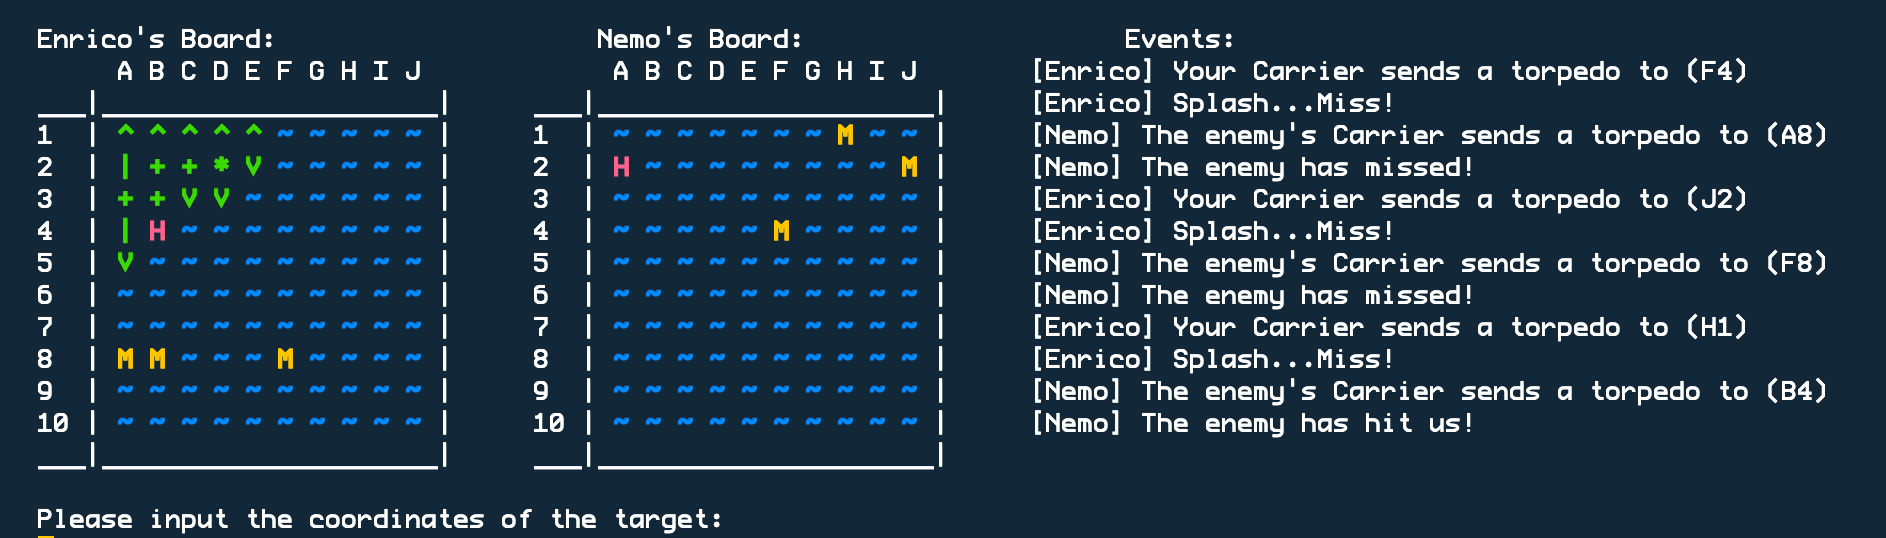
\includegraphics[scale=0.55]{images/game.png}
\caption{Screenshot of the game view after a few turns between a human and computer player.}
\label{fig:game_view}
\end{figure}

\subsection{Memory and Smart Pointers}
The use of smart pointers was employed throughout to ensure no memory leaks occurred, or at least minimise the possibility
this might happen.
Namely:
\begin{enumerate}[label=\roman*.]
  \item The board class uses a unique pointer to the array of strings containing the board representation at every
  coordinate. Moreover, it has a member vector of unique pointers to pieces held by the board.
  \item The main method uses shared pointers to players since these will then be assigned to each player as an enemy.
  \item Following this, each player holds a weak pointer to each other as an enemy.
   This prevents reference cycles from denying the player pointers to be dereferenced on deletion.
\end{enumerate}
To check that no memory leaks were present, the program was run for all possible
routines while using Valgrind (an opensource memory leak debugger) in the background
and the complete log can be found in Appendix 3 detailing that
\textbf{no memory leaks were found}.
\section{Results}
The following is a single run of the game visualised through screenshots of
 the most important screens and menus.
\begin{figure}[H]
\centering
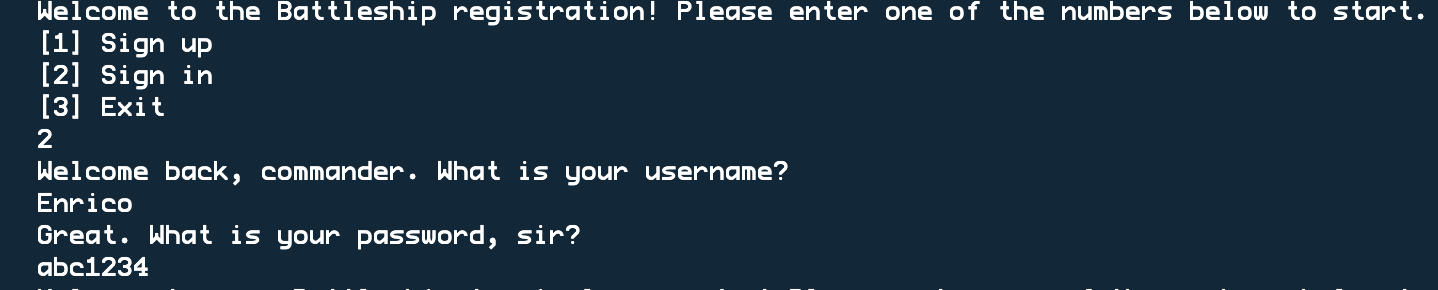
\includegraphics[scale=0.5]{images/login_screen.png}
\caption{Screenshot of the first menu when launching the program for login/signup.}
\end{figure}
\begin{figure}[H]
\centering
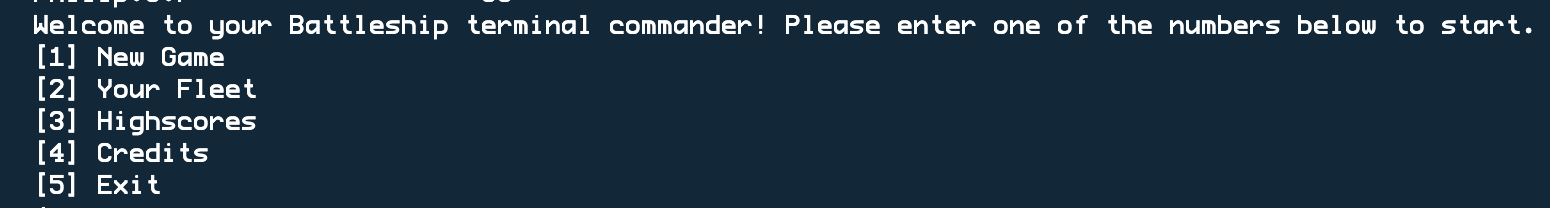
\includegraphics[scale=0.5]{images/main_screen.png}
\caption{Screenshot of the main menu from which different routines are launched.}
\end{figure}
\begin{figure}[H]
\centering
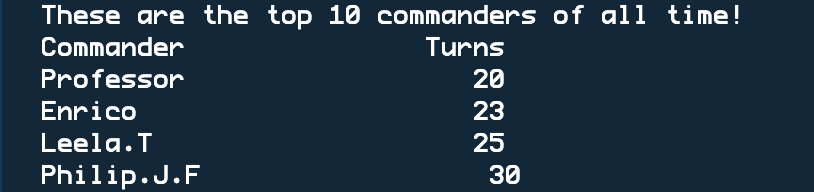
\includegraphics[scale=0.5]{images/highscores.png}
\caption{Screenshot of the all-time highscores panel.}
\end{figure}
\begin{figure}[H]
\centering
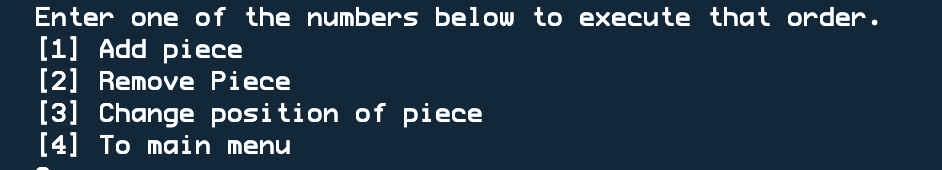
\includegraphics[scale=0.5]{images/edit_screen.png}
\caption{Screenshot of the fleet editing menu.}
\end{figure}
\begin{figure}[H]
\centering
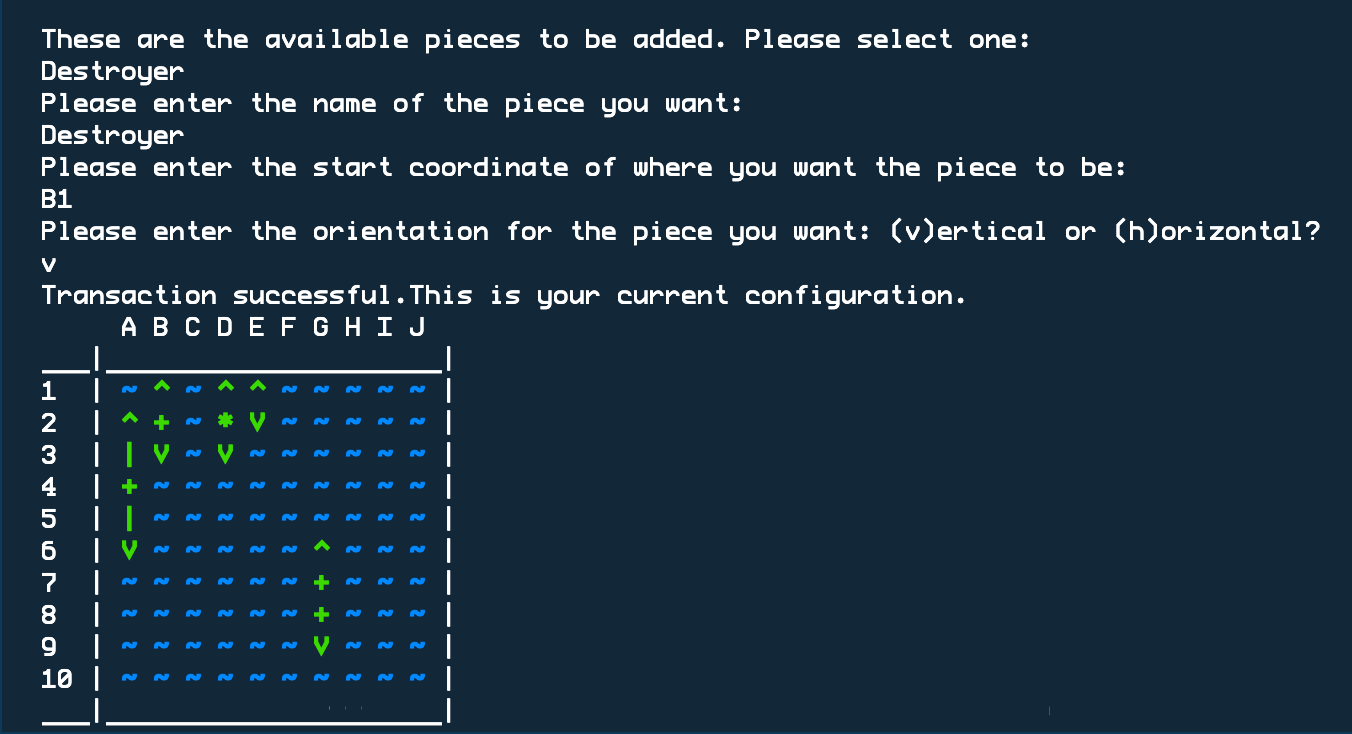
\includegraphics[scale=0.5]{images/add_piece.png}
\caption{Screenshot of adding pieces to fleet, if not all the pieces have been added already.}
\end{figure}
\begin{figure}[H]
\centering
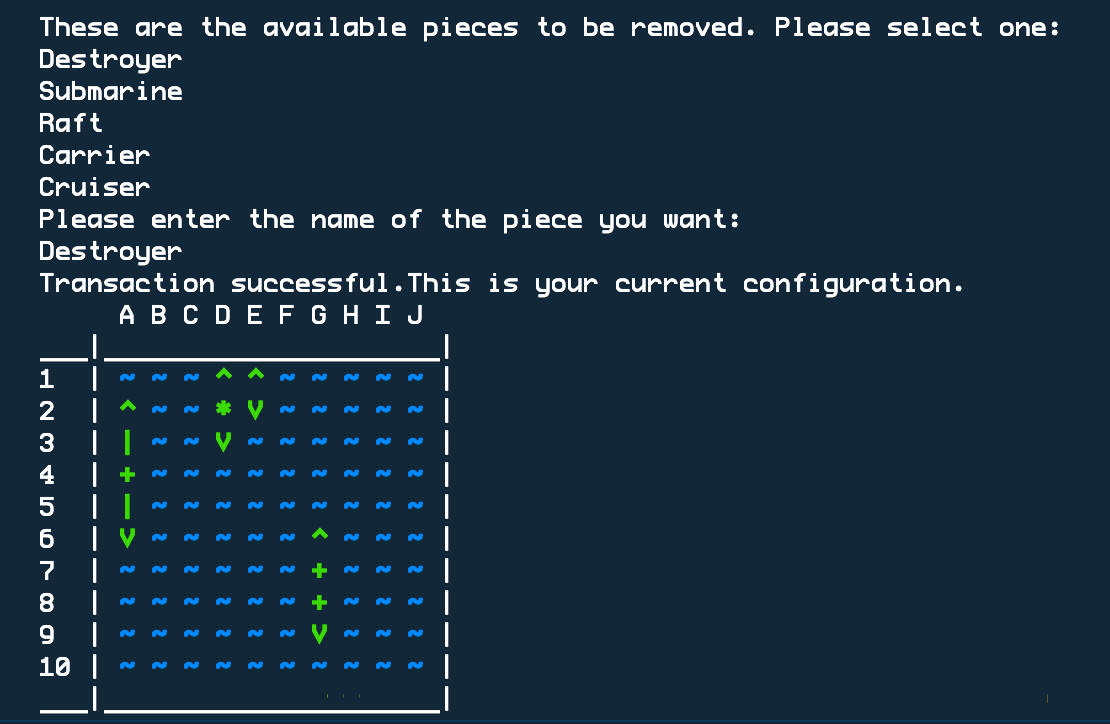
\includegraphics[scale=0.5]{images/delete_piece.png}
\caption{Screenshot of deleting a piece from the fleet, if the fleet is not empty.}
\end{figure}
\begin{figure}[H]
\centering
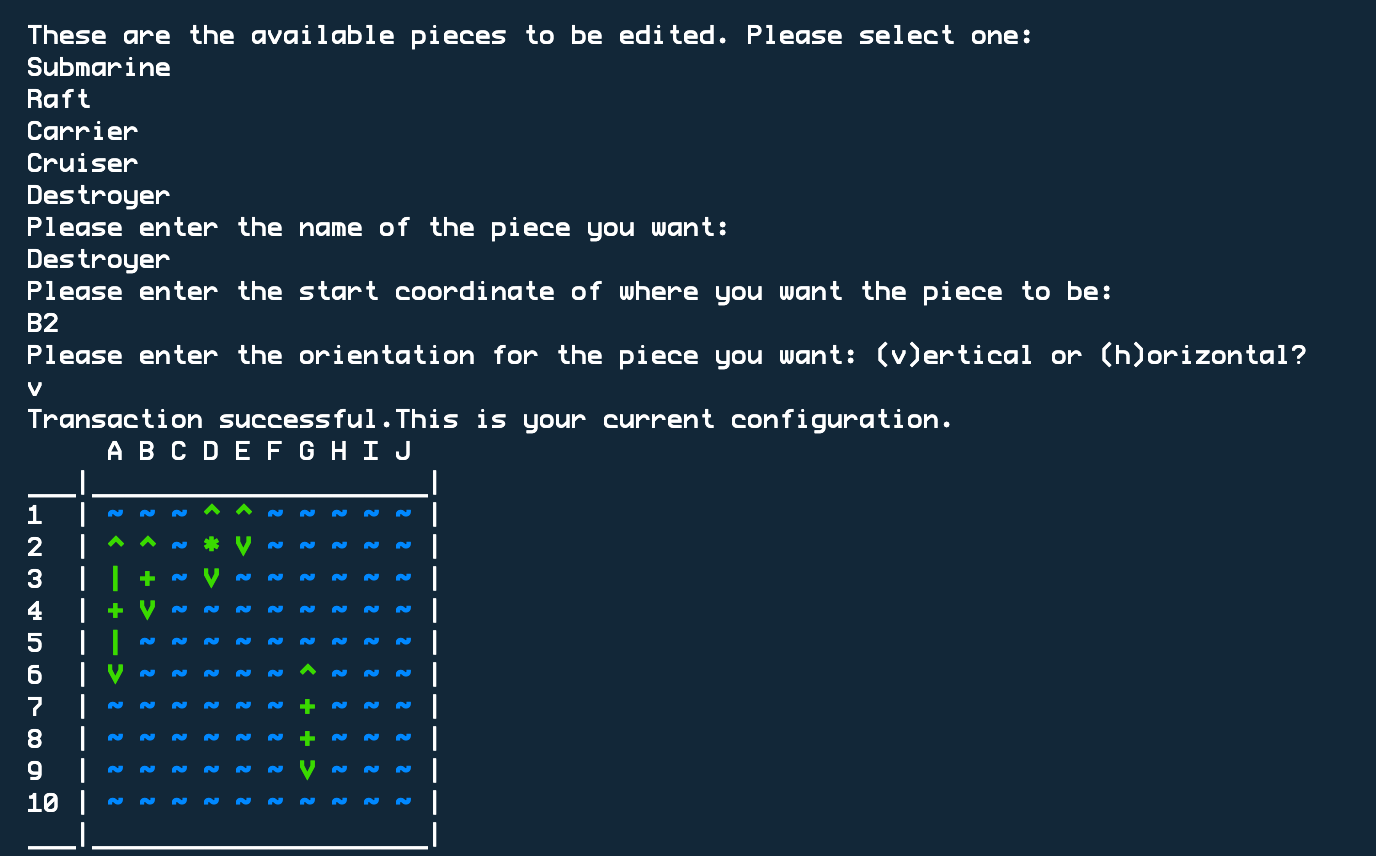
\includegraphics[scale=0.5]{images/change_pos.png}
\caption{Screenshot of changing position of a piece in the fleet.}
\end{figure}
\begin{figure}[H]
\centering
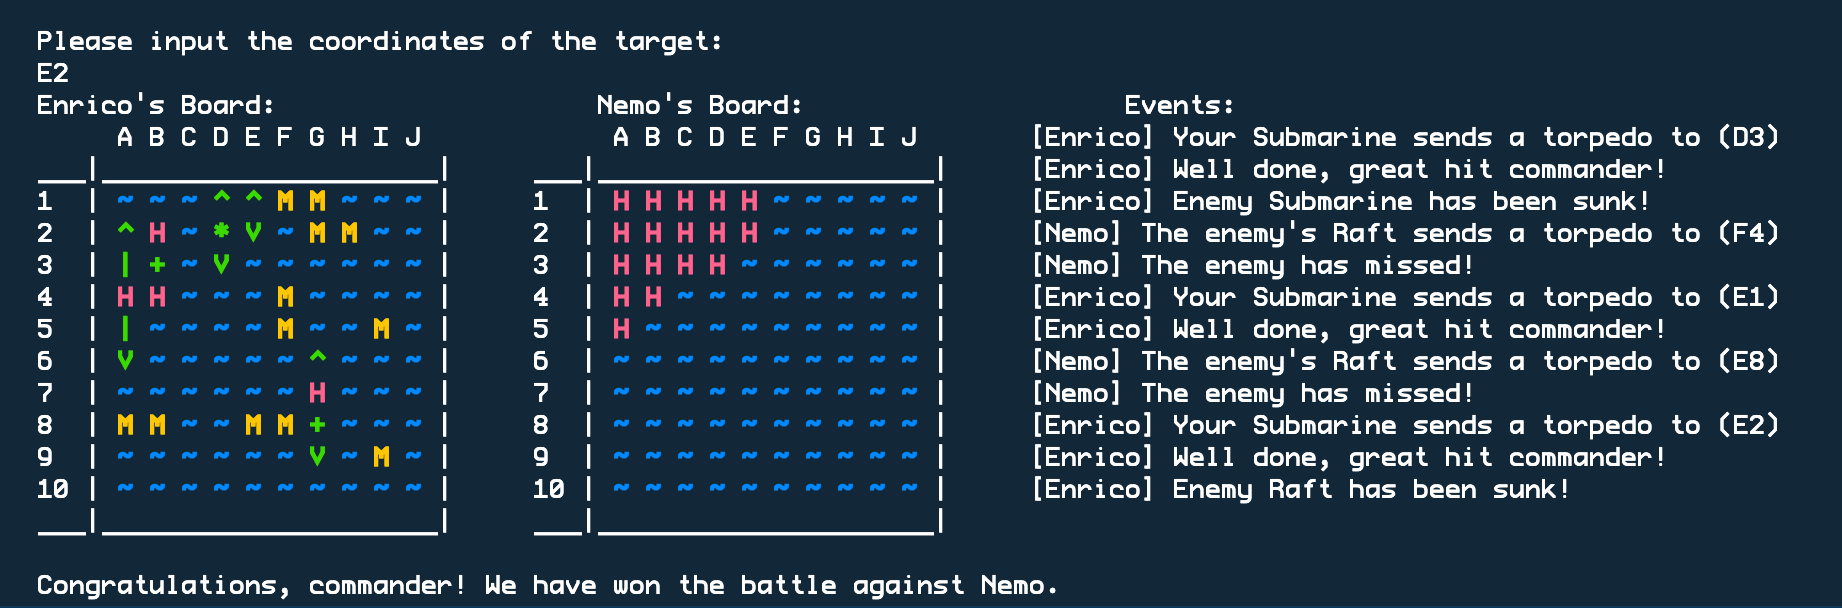
\includegraphics[scale=0.5]{images/win_game.png}
\caption{Screenshot of winning the game against the NPC.}
\end{figure}
\section{Conclusions and Extensions}
All required functionality set out at the beginning in Section 1.3 was completed successfully.
The whole program was tested for input validation and sanitization
together with memory checks to make sure no leaks occur.
Finally, object oriented features such as inheritance, polymorphism,
encapsulation and abstraction were all implemented.
Advanced C++ features such as the use of generic lambda functions, hashmaps,
tuples and all three types of smart pointers were used.
\\
\par As possible extensions, even though currently every piece has the same cost i.e 1 and the budget each player has is the number of pieces,
one could very easily change this in the future by constraining the budget and maybe adding more vessels with different costs
opening a really big game element such as is choosing your fleet correctly.
Moreover, since the game saves fleet state after closing, creating one's fleet wisely has even more value.
Finally, implementing a smarter NPC strategy than random selection would be interesting possibly with
different levels of opponent difficulty too.
\\
\par \hfill 2480 words\\
\printbibliography
\newpage
\section*{Appendix 1: Impact of COVID19 on the work completed and report}
\subsection{Time lost travelling home}
On the 16th of March I caught the first airplane home (Malta) I could find, due to news that airports back home were soon closing.
As a matter of fact a week later they did close permanently and so have the UK soon after that.
The time I did lose was not explicitly in travelling home although that was substantial (around 10 hours all together)
it was more since I left almost imminently I left a lot of resources back in Manchester (such as books, documents) and it has
been really painful trying to find alternatives to them.
\subsection{Lack of access to computers and the internet}
I am very lucky to have no problem on this end since I have a laptop I could take with me and
I have a stable internet connection.
In fact I attended all the lectures on BlackBoard Collaborate that occurred for this and other modules.
\subsection{Limitation in the outcome}
I honestly do not think it has affected me in any way towards this particular module.
The lecturer and lab assistants all have been very helpful online whenever I needed and learning resources, perhaps
because this is a programming module, were fairly easy to find online.
\section*{Appendix 2: Instructions for Opening Optional Full Documentation}
Attached to the .cpp and .h files should be a directory called html.
This directory is not required to run the program but rather is a fully
compiled documentation of the whole code.
It is a nice, UI friendly way to check the codebase.
The way to open it is to enter the directory and open the file 'index.html'
in a browser.
\newpage
\section*{Appendix 3: Log of Valgrind Memory Check}
{\obeylines\obeyspaces
\texttt{
\input{valgrind-out.txt}
}}

\end{document}
